\chapter{Style and content}\label{chap:style}
Although the model presented in Chapter~\ref{chap:architecture} learns to model SVGs from a single class, it encodes style and content together in its latent space.
Here, we investigate a modified classifying architecture that explicitly encodes content separately and report experiment results.

\section{Model architecture}
\begin{figure}[h]
\centering
\caption[An overview of the SVG model architecture with explicit label encoding]{An overview of the SVG model architecture with explicit label encoding.
\label{fig:label-arch}}
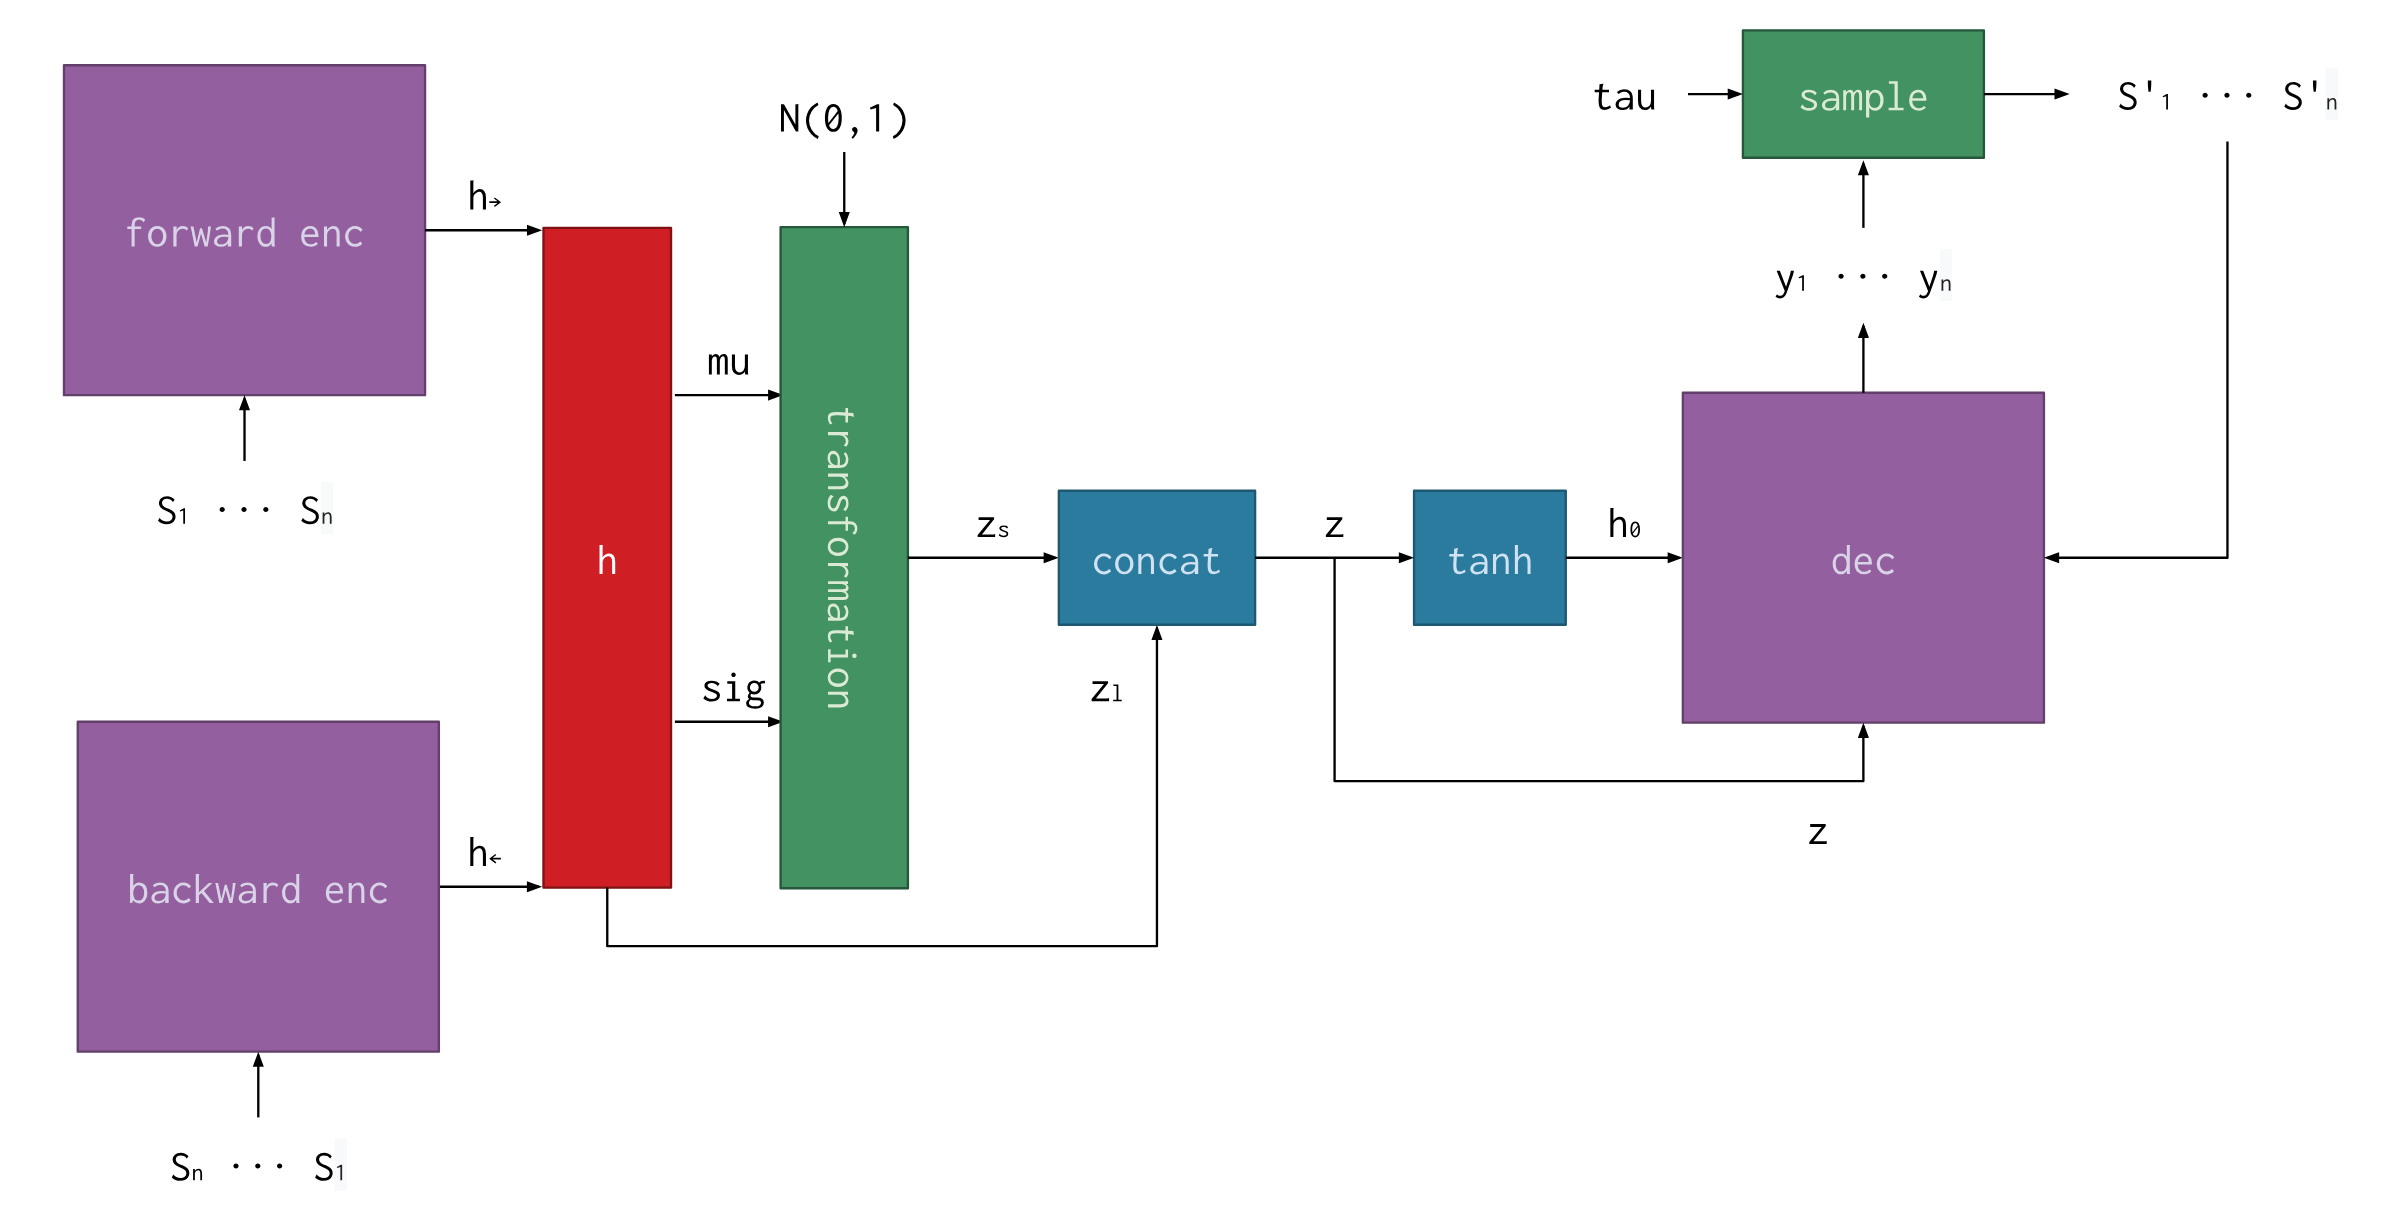
\includegraphics[width=\textwidth]{figures/label_architecture}
\end{figure}

The model presented originally transforms the final layer of the encoder RNN into $\mu$ and $\sigma$ vectors, which are then combined with random $\mathcal{N}(0,1)$ samples to form a latent space vector $z$.

We modify this architecture to also generate a label vector $z_l$ from the encoder's final layer that models a categorical distribution over input classes.
Assuming there are $n_c$ input classes and a latent space dimension of $n_z$, we adjust $\mu$ and $\sigma$ to be of dimension $n_z - n_c$, then perform the same transformation to generate $z_s$.
We concatenate these two vectors, $z_l$ and $z_s$, to form $z$, which is then fed into the decoder as before.

Finally, we add another term in the loss function representing the log loss of the label prediction with the ground truth label (encoded as a $n_c$-dimensional one-hot vector).
With the ground truth label encoded as $(c_1, \cdots, c_{n_c})$, the log loss of label prediction is:

\begin{equation}
L_c = \sum_{i=1}^c c_i \log(z_{li})
\end{equation}

\section{Classifying experiment}
\begin{figure}[h]
    \centering
	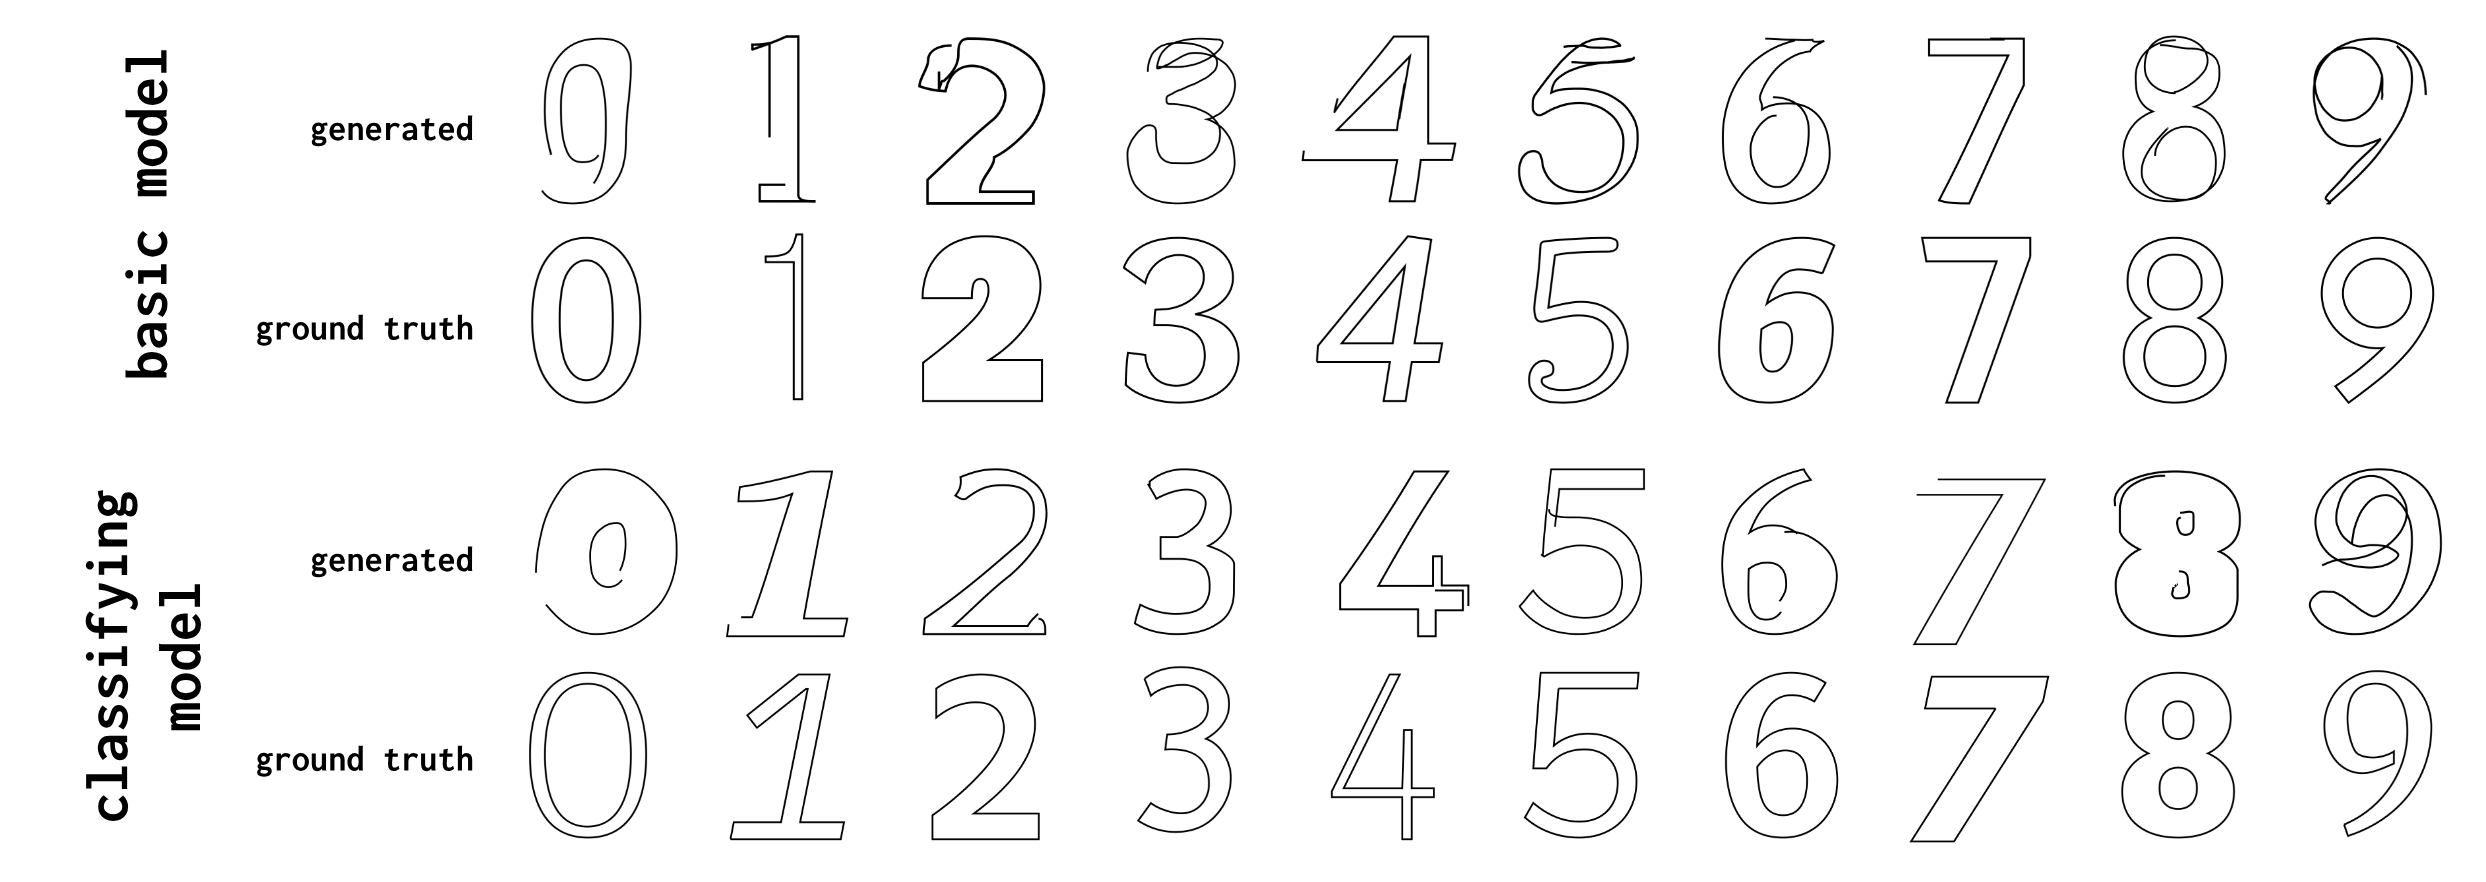
\includegraphics[width=\textwidth]{figures/digits}
    \caption[Visual results for the multi-class digits models]
    {Selected conditionally generated digits from the models in Section~\ref{sec:class-exp} trained on a multi-class dataset.\label{fig:class-results}}
\end{figure}

We perform an experiment comparing two models: one version of the original model and one version of the classifying model.
To generate a multi-class dataset, we combine datasets for the digit glyphs (i.e. digits 0 through 9).
Input SVGs are encoded using encoding B as described in Chapter~\ref{chap:feature-variation}.
Overall, the resulting dataset has 20k training examples, 2.4k test examples, and 2.4k validation examples.

Both models were trained for 450k iterations with the same parameters as models described in Chapter~\ref{chap:training}, and details about training loss can be found in Appendix~\ref{app:train}.

\section{Results}
In conditionally recreating input images, we find that the models are comparable, with the original model performing slightly better in quantitative evaluation. Selected decoded outputs from both models are shown in Figure~\ref{fig:class-results}.

\begin{table}[h]
\centering
\caption[Quantitative results for evaluating multi-class models]
    {Modified Hausdorff distance for models trained on the digit glyph dataset with each encoding on a test set of $N$ images.\label{tbl:class-results}}
\begin{tabular}{c c c c c}
\toprule
    Model & Mean & Std.\ dev. & Kurtosis & $N$ \\ \midrule
    Original & 25.5308 & 10.5062 & 3.1082 & 2400 \\
    Modified & 26.6192 & 16.9867 & 15.8120 & 2326
\end{tabular}
\end{table}

We evaluate results quantitatively by computing the Hausdorff similarity metric between each ground-truth test set image and a corresponding image conditionally generated by the model with $\tau = 0.1$, using the same method as described in Section~\ref{sec:quant-eval}. Results are reported in Table~\ref{tbl:class-results}.

\begin{table}[h]
\centering
\caption[Classification accuracy for the modified multi-class model]
    {Classification accuracy for the modified multi-class model.\label{tbl:class-acc}}
\begin{tabular}{c c}
\toprule
    Digit & Classification accuracy \\ \midrule
    0 & 82.08\% \\
    1 & 41.25\% \\
    2 & 92.91\% \\
    3 & 97.08\% \\
    4 & 49.16\% \\
    5 & 56.66\% \\
    6 & 61.25\% \\
    7 & 80.83\% \\
    8 & 95.83\% \\
    9 & 88.33\%
\end{tabular}
\end{table}

Finally, we report the classification accuracy from the modified model, generated by comparing the highest probability predicted class to the ground truth class. The classifying model has an overall accuracy of 74.54\%, with accuracy rates per class reported in Table~\ref{tbl:class-acc}.

One factor that may partially explain the classifying model's lack of improvement in generating conditional images over the basic model is the reduced latent vector size.
Both models set $n_z$ to be 128, but the basic model is able to use the entire latent vector to encode the input drawing, while the classifying model must reserve 10 dimensions for the digit class vector.
Future work can explore this hypothesis as well as experiment with other adjustments to the model architecture to further improve performance.

\section{Style transfer}
We verify that the class encoding is used by the decoder by manually substituting out the portion of $z$ corresponding to $z_c$ with a different class encoding.
Although we did not quantitatively evaluate these results, we report visual results for more common font styles in Figure~\ref{fig:style-trans}. 

\begin{figure}[h]
    \centering
	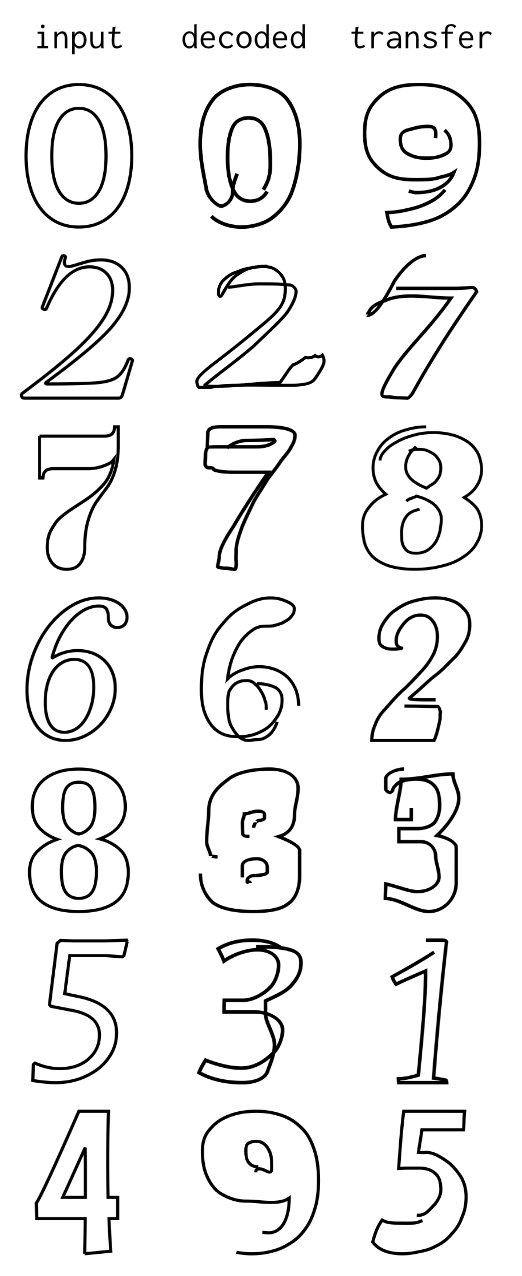
\includegraphics[height=0.9\textheight]{figures/style_trans}
    \caption[Examples of style transfer using the classifying model]
    {Examples of style transfer using the classifying model.
    Outputs were decoded at $\tau=0.1$.
    In the last two rows, the model misclassified the inptu 5 as 3 and the input 4 as 9, resulting in the incorrect decoded output.
    \label{fig:style-trans}}
\end{figure}
